\documentclass[10pt]{article}

%si colocas esto se ve en times new roman, pero compilas es con xelatex
%\usepackage{fontspec}
%\setmainfont{Times New Roman}

\usepackage{tocbibind}

\usepackage[a4paper]{geometry}
\geometry{top=2.54cm, bottom=2.54cm, left=2.54cm, right=2.54cm}
\usepackage[spanish]{babel}

\usepackage{float}
\usepackage{graphicx} % graficos
\graphicspath{ {./images/} }
\usepackage{setspace}%interlineado agrega:
\usepackage{listings}
\usepackage{xcolor}
\usepackage{fancyvrb}
\definecolor{codegreen}{rgb}{0,0.6,0}
\definecolor{codegray}{rgb}{0.5,0.5,0.5}
\definecolor{codepurple}{rgb}{0.58,0,0.82}
\definecolor{backcolour}{rgb}{0.95,0.95,0.92}

\lstdefinestyle{mystyle}{
    backgroundcolor=\color{backcolour},
    commentstyle=\color{codegreen},
    keywordstyle=\color{magenta},
    numberstyle=\tiny\color{codegray},
    stringstyle=\color{codepurple},
    basicstyle=\ttfamily\footnotesize,
    breakatwhitespace=false,
    breaklines=true,
    captionpos=b,
    keepspaces=true,
    numbers=left,
    numbersep=5pt,
    showspaces=false,
    showstringspaces=false,
    showtabs=false,
    tabsize=2
}

\lstset{style=mystyle}
% \doublespacing \onehalfspace \singlespace \spacing{x}
\spacing{1.5}
\pagestyle{headings}

\usepackage[backend=biber, autocite=inline, labeldateparts=true, maxcitenames=1,style = apa]{biblatex}
\bibliography{referencias}

\usepackage{csquotes}
\usepackage[bookmarks = true, colorlinks=true, linkcolor = black, citecolor = black, menucolor = black, urlcolor = black]{hyperref}

\newcommand{\comillas}[1]{``#1"}

\begin{document}
\renewcommand{\listtablename}{Índice de Tablas}
\pagenumbering{roman}

	\setcounter{page}{0}
\begin{titlepage}

\begin{table}[t]
\centering
\begin{tabular}{ p{3cm} p{8.5cm} p{3cm} }
	\begin{flushleft}
\includegraphics[width=2.4cm]{logo_poli.png}\end{flushleft} &



	\begin{center}
	República Bolivariana de Venezuela\\
	Universidad Nacional Experimental Politécnica “Antonio José de Sucre”\\
	Vice Rectorado Barquisimeto \\
	Departamento de Ingeniería Electrónica\\  

%***************************************************
%************** aqui va el titulo ******************
%***************************************************

	\vspace*{65mm}
	\begin{LARGE}
		Practica 3\\ laboratorio de diseño de sistemas de computación
	\end{LARGE}

	\end{center}


	& \begin{flushright}
\includegraphics[width=1.7cm]{logo_electronica.jpg} \end{flushright}
\end{tabular}


	\vspace*{3mm}

	\parbox[c]{12cm}{
	\begin{center}
		\begin{small}
			
		\end{small}
	
	\end{center}
	}

	
	
	\vspace*{45mm}



\begin{flushright}
Integrantes:\\


Gerardo Alfonzo Campos Fonseca\\ 
V. 27085179\\
José Andrés Cortez Teran\\
V. 26540824\\

\vspace*{2mm}


\end{flushright}
\vspace*{5mm}

\begin{center}Barquisimeto, Julio del 2021\end{center}
\end{table}
\end{titlepage}



	\newpage
	\tableofcontents
	\newpage
	\listoffigures
	%\newpage
	%\listoftables


    %\newpage
    \pagenumbering{arabic}
	%***************************************************************************
%*************** PRIMERA PARTE *********************************************
\section{Primera Actividad}

\subsection*{1.7}
Se creo un único archivo \textbf{mensaje.obj}, el cual es un archivo de tipo ``objeto''.

\begin{figure}[H]
  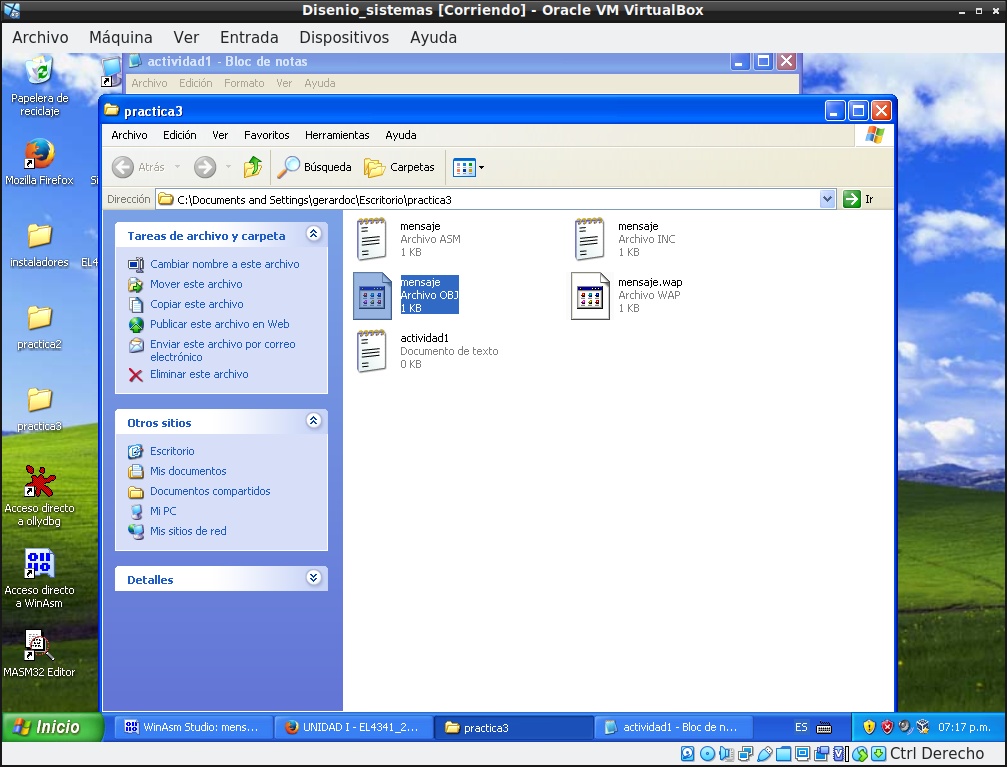
\includegraphics[width=\linewidth]{practica3/imagenes/actividad1/creados_compilacion.png}
  \caption{archivos creados al compilar}
\end{figure}

\subsection*{1.8}
Se creo un único archivo, el ejecutable \textbf{mensaje.exe}.

\begin{figure}[H]
  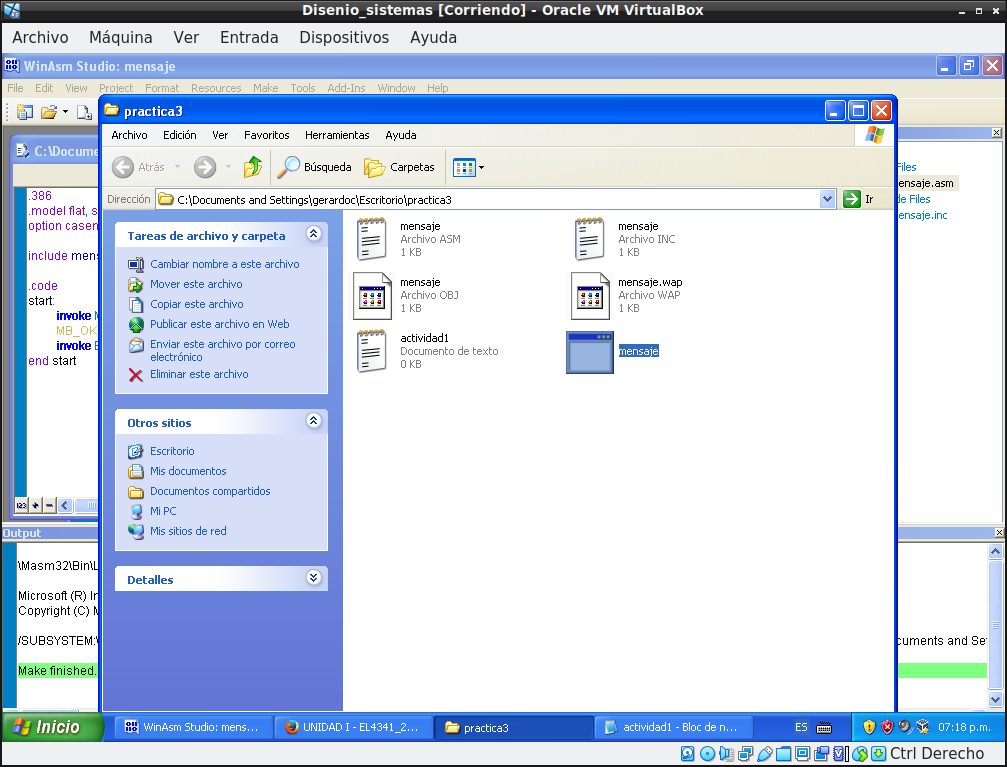
\includegraphics[width=\linewidth]{practica3/imagenes/actividad1/creados_link.png}
  \caption{archivos creados al enlazar}
\end{figure}

\subsection*{1.9}
Al ejecutar el programa se abre una ventana de mensajes (ventana emergente), la cual dice: ``Este es un programa simplea para Windows'' y se cierra al presionar el boton ``Aceptar''.

\begin{figure}[H]
  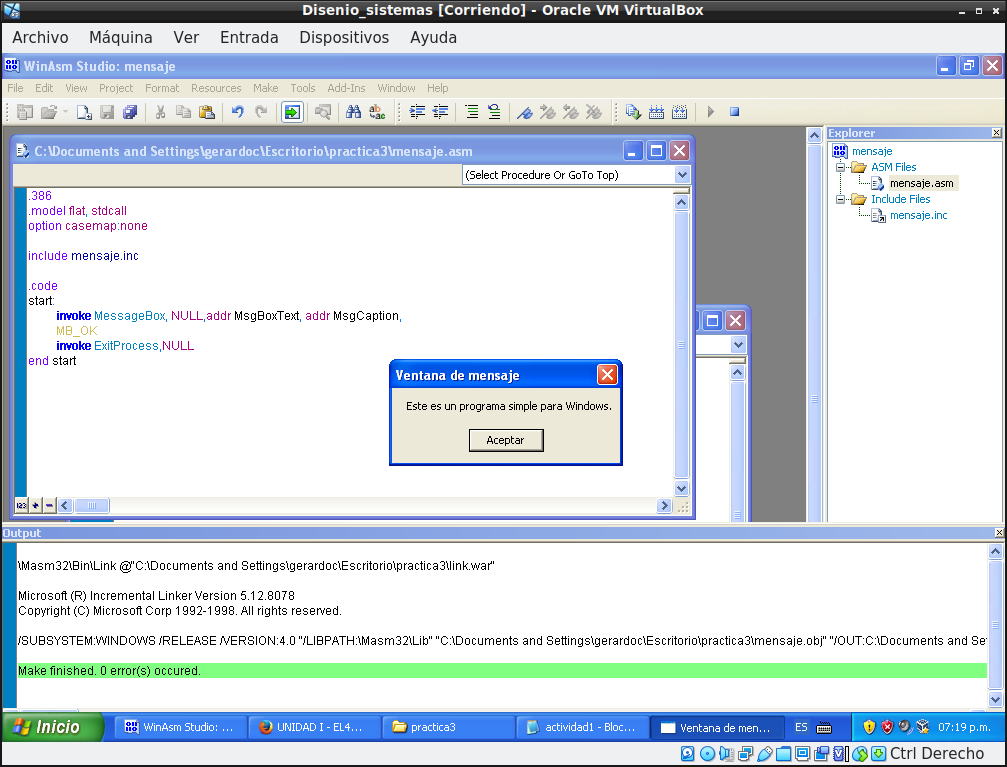
\includegraphics[width=\linewidth]{practica3/imagenes/actividad1/ejecucion.png}
  \caption{ejecución del programa}
\end{figure}

%***************************************************************************
%*************** SEGUNDA PARTE *********************************************
\section{Segunda Parte}

\begin{figure}[H]
  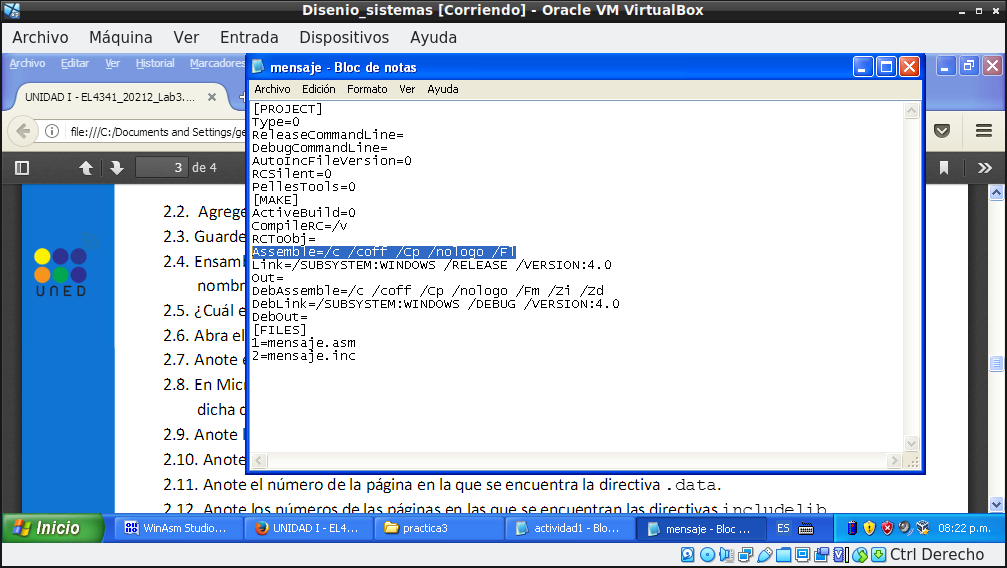
\includegraphics[width=\linewidth]{practica3/imagenes/actividad2/edicion_proyecto.png}
  \caption{edición del proyecto}
\end{figure}

\subsection*{2.4}
Se usa el comando:

\begin{BVerbatim}

\Masm32\Bin\ML /c /coff /Cp /nologo /Fl /I"\Masm32\Include"
"C:\Documents and Settings\gerardoc\Escritorio\practica3\mensaje.asm"

\end{BVerbatim}

Los archivos que se crearon fueron:

\begin{itemize}
    \item \textbf{mensaje.obj} (igual que anteriormente)
    \item \textbf{mensaje.lst}
\end{itemize}

\begin{figure}[H]
  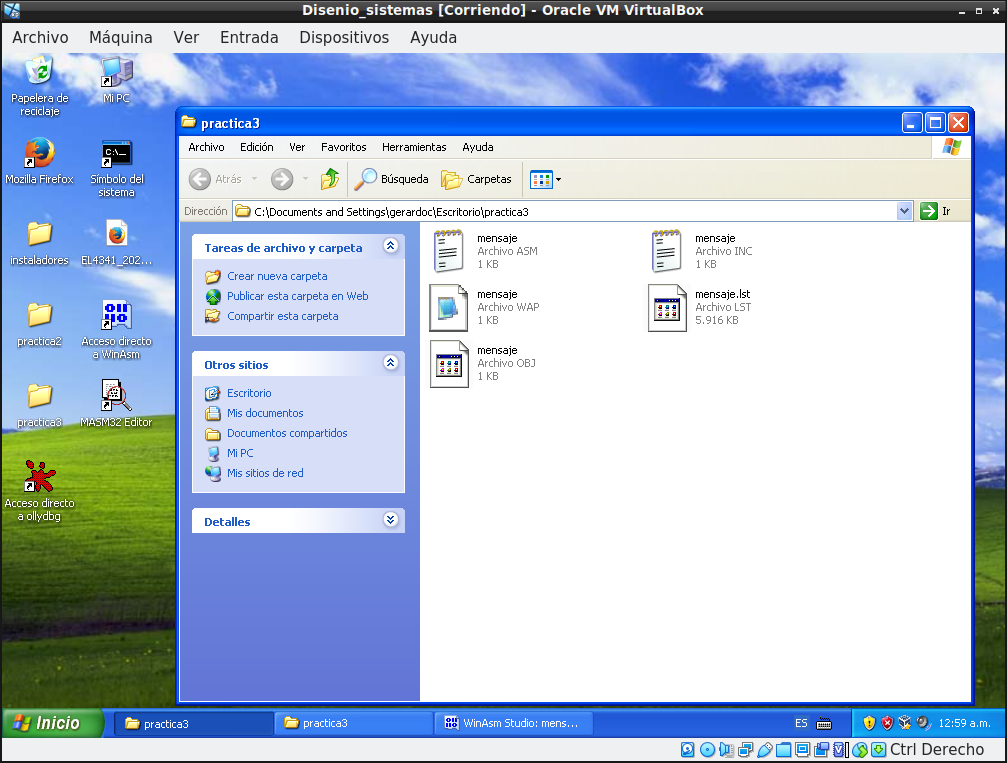
\includegraphics[width=\linewidth]{practica3/imagenes/actividad2/archivos_compilacion.png}
  \caption{archivos creados al compilar}
\end{figure}

\subsection*{2.5}
La opción \textbf{/Fl} se utiliza para generar una lista de código ensamblado (Generates an assembled code listing).

\subsection*{2.7}
El archivo ocupa 2752 paginas, Cabe resaltar que se uso \textbf{Libreoffice  Writer}.

\begin{figure}[H]
  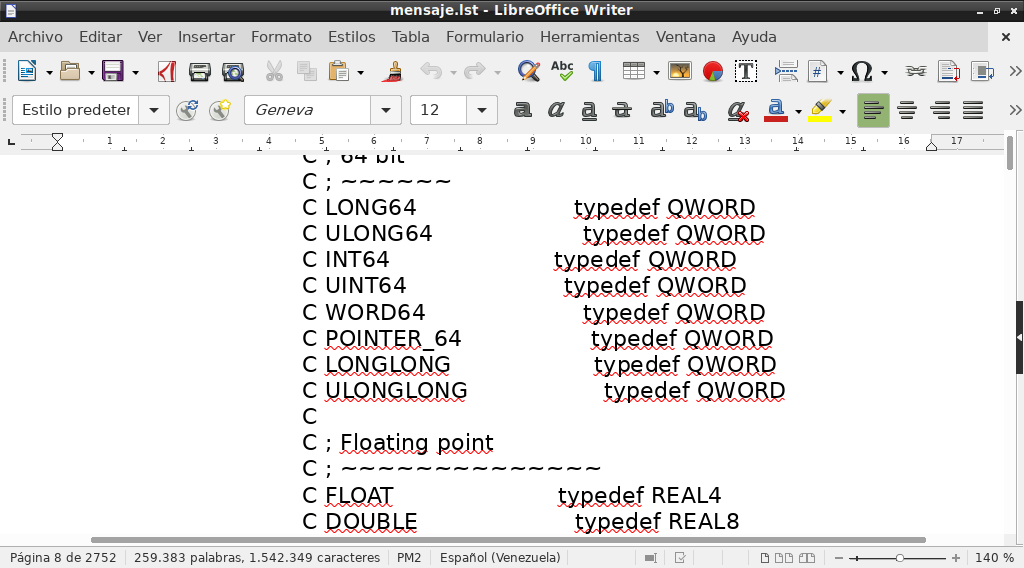
\includegraphics[width=\linewidth]{practica3/imagenes/actividad2/mensaje_lst_word.png}
  \caption{Numero de paginas}
\end{figure}

\subsection*{2.8}
La directiva \textbf{end start} se encuentra en la pagina 1638.

\subsection*{2.9}
Las dos instrucciones que comienzan con \textbf{invoke} se encuentran en la pagina 1638.

\subsection*{2.10}
La directiva \textbf{.code} se encuentra en la pagina 1638.

\subsection*{2.11}
La directiva \textbf{.data} se encuentra en la pagina 1638.

\subsection*{2.12}
Ambas directivas \textbf{includelib} se encuentra en la pagina 1638.

\subsection*{2.13}
Las directivas se encuentran en:

\begin{itemize}
    \item \textbf{include windows.inc} en la pagina 1.
    \item \textbf{include kernel32.inc} en la pagina 1531.
    \item \textbf{include user32.inc} en la pagina 1591.
\end{itemize}

\subsection*{2.14}
La directiva include \textbf{mensaje.inc} esta en la pagina 1.

\subsection*{2.15}
Inserta código fuente, del archivo de código fuente proporcionado por
\textbf{filename}, en el archivo de código fuente actual durante el ensamblado.


%***************************************************************************
%*************** Tercera PARTE *********************************************
\section{Tercera Parte}

\begin{figure}[H]
  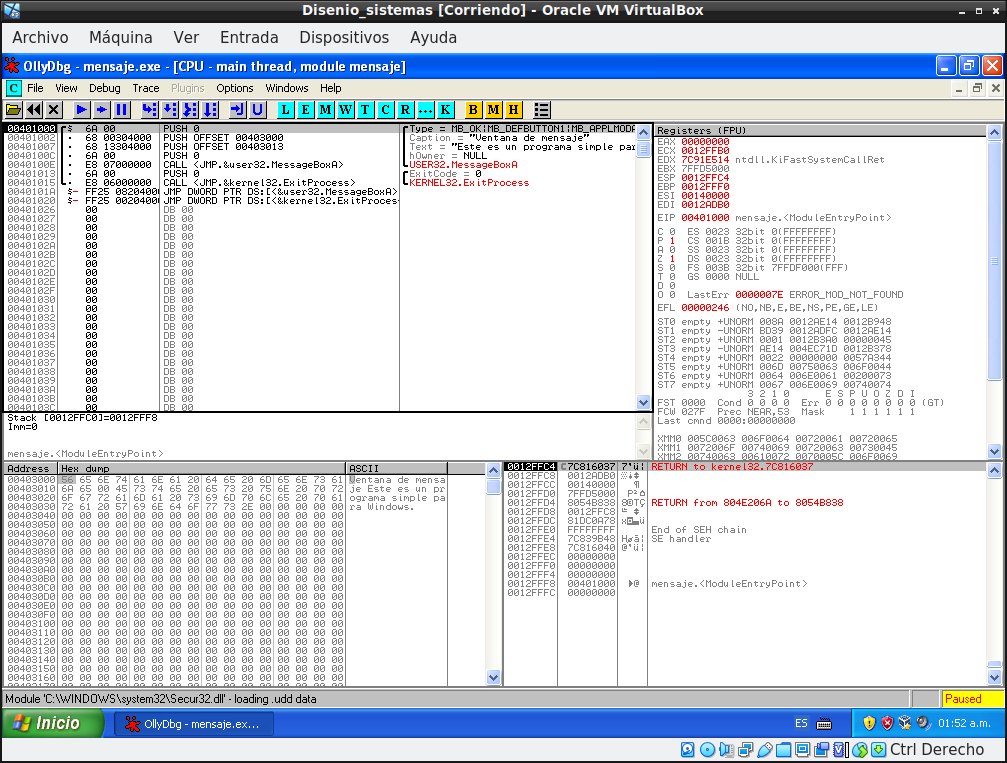
\includegraphics[width=\linewidth, scale=0.9]{practica3/imagenes/actividad3/olly.png}
  \caption{Ejecutable en Olly}
\end{figure}

\subsection*{3.2}
La primera instrucción según \textbf{Olly} es \verb|PUSH 0|.

\subsection*{3.3}
La dirección de la primera instrucción es 00401000 y le da el nombre de
\verb|mensaje.<moduleEntryPoint>|.

\subsection*{3.4}
Las lineas dicen:

\begin{itemize}
    \item \textbf{MessageBox:} dice: \verb|Dest = mensaje.0040101A - jumps to user32.MessageBoxA| y se lee la direccion a la que saltara en: \verb|mensaje.<moduleEntryPoint>+0E|.
    \begin{figure}[H]
      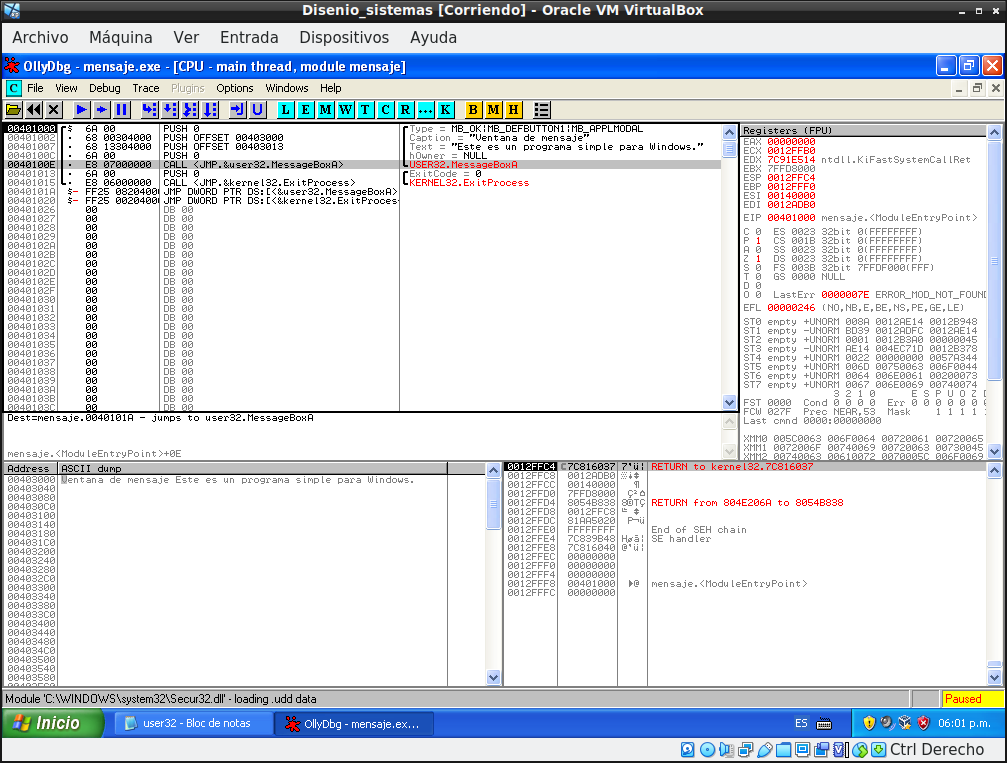
\includegraphics[width=\linewidth, scale=0.9]{practica3/imagenes/actividad3/message.png}
        \caption{Ejecutable en Olly, MessageBoxA instruction}
    \end{figure}

\item MessageBox: dice: \verb|Dest = mensaje.00401020 - jumps to Kernel32.ExitProcess| y se lee la direccion a la que saltara en: \verb|mensaje.<moduleEntryPoint>+15|.
    \begin{figure}[H]
      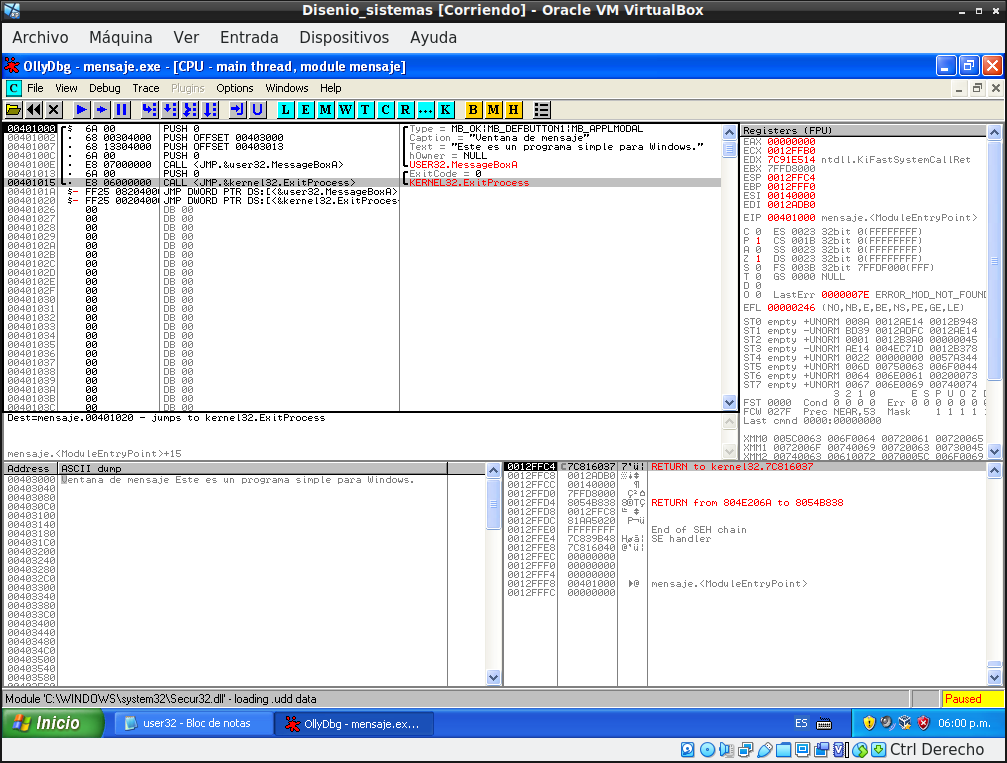
\includegraphics[width=\linewidth, scale=0.9]{practica3/imagenes/actividad3/exit.png}
      \caption{Ejecutable en Olly, ExitProcess instruction}
    \end{figure}
    \end{itemize}

\subsection*{3.5}
Según \cite{MicrosoftINVOKE} es una directiva que solo funciona con \textbf{MASM} de 32
bits y llama al procedimiento de la dirección proporcionada por la expresión,
puede contener argumentos y todo esto es pasado por la pila o en registros,
según sean las convenciones de llamada estándar del lenguaje. Se usa de la
forma \verb|INVOKE expresion [,argumento, \dots]|.

%***************************************************************************
%*************** CUARTA PARTE *********************************************
\section{Cuarta Parte}

\subsection*{4.1}

Debido a que no se encontró el archivo \textbf{win32.hlp}, se busco en
internet y consiguió \textbf{win32.chm} en \cite{laurencejackson.com}. La cual es versión
actualizada del sistema de ayudas de Windows, pero de todas formas contiene
la misma información.

\subsubsection*{MessageBox}

La función \textbf{MessageBox} crea, muestra y opera una caja de mensaje. El \textbf{MessageBox}
contiene un mensaje definido en la aplicación, un titulo y un numero predefinido
de iconos y botones.

\begin{BVerbatim}

int MessageBox(
HWND hWnd, // handle of owner window
LPCTSTR lpText, // address of text in message box
LPCTSTR lpCaption, // address of title of message box
UINT uType // style of message box
);

\end{BVerbatim}

\subsubsection*{ExitProcess}

La función ExitProcess termina el proceso y todos sus hilos de ejecución.

\begin{BVerbatim}

VOID ExitProcess(
UINT uExitCode // exit code for all threads
);

\end{BVerbatim}

\subsection*{4.2}
La linea es:  \verb|ExitProcess PROTO STDCALL :DWORD|.

\subsection*{4.3}
\textbf{MessageBoxA} aparece en la definición y todo es:

\begin{BVerbatim}

MessageBoxA PROTO STDCALL :DWORD,:DWORD,:DWORD,:DWORD
IFNDEF __UNICODE__
  MessageBox equ <MessageBoxA>

\end{BVerbatim}


\section*{Post}

\subsection*{1.}

Una interfaz para programación de aplicaciones, como su nombre lo indica, es
una interfaz que facilita la elaboración de aplicaciones. Las aplicaciones de
Windows necesitan hacer llamadas al núcleo del sistema operativo. Como estas
funcionalidades pueden cambiar entre diferentes versiones del sistema
operativo, Microsoft elaboro la \textbf{API} de windows. El \textbf{API}
proporciona una interfaz estándar, que mantiene retrocompatibilidad mientras
que permite cambiar su implementación en diferentes versiones del sistema
operativo. Ademas, el \textbf{API} también ayuda al programar proporcionando
funciones que facilitan tareas comunes en la programación de aplicaciones.

\subsection*{2.}

Una biblioteca de enlace dinámico es un conjunto de funciones que son cargadas
por una aplicación en tiempo de ejecución. Esto lo diferencia de las
bibliotecas estáticas que son enlazadas en tiempo de compilación. Esto trae
múltiples ventajas y múltiples desventajas. La principales ventajas son que
disminuye el tamaño del ejecutable y que la actualización de las librerías no
requiere una actualización de las aplicaciones. Las principales desventajas son
que tiene una penitencia en tiempo de ejecución y que son vector de ataque para
\textbf{hackers}, los cuales pueden insertar un \textbf{DLL} malicioso en una
aplicación con privilegios.

\subsection*{3.}

Según el articulo \cite{MicrosoftDLL} \textbf{Kernel32.dll} posee funciones
de bajo nivel para manejar recursos del sistema operativo, como el manejo
de memoria y creación de procesos ; \textbf{GDI32.dll} posee funciones para
el manejo de dispositivos de salida, como puede ser el dibujar en pantalla
o el manejo de fuentes tipográficas y  \textbf{User32.dll} tiene funciones para
el manejo de temporizadores, menús y comunicaciones.

\subsection*{4.}

El prototipo de una función indica que parámetros toma la función y que tipo
de dato retorna. Tienen la siguiente estructura:

\begin{center}
\begin{BVerbatim}

    ValorDeRetorno nombreDeFuncion(TipoDato1 param1, ....){
        // Información adicional del cuerpo de la funcion
    }
\end{BVerbatim}
\end{center}

\subsection*{5.}

Una archivo que contiene declaraciones, cabeceras, funciones y otros
datos relacionados a un librería. Son equivalentes a los archivos \textbf{.h}
de C.

\subsection*{6.}

Contiene la implementación de funciones declaradas en los \textbf{.inc}, son
la contraparte estatica de los \textbf{.dll}. Son archivos binarios que
contienen codigo compilado de un lenguaje de alto nivel o código ensamblado.

\subsection*{7.}

Ambas son librerías (conjunto de funciones o datos reutilizables), la diferencia
esta en su forma de enlazado. En las librerías estáticas el proceso de enlazado
ocurre en la etapa de compilación, mientras que en las librerías dinámicas
el enlazado ocurre en tiempo de ejecución.

\subsection*{8.}

La directiva \textbf{INVOKE} es un poderoso reemplazo para las instrucciones
\textbf{CALL} de intel, ya que deja pasar múltiples argumentos de una forma mas
sencilla. Por tanto, se encarga de llamar procedimientos que se encuentren en
una dirección dada, definida por una \textbf{expresión}, y pasarle los
parámetros necesarios.  Maneja argumentos de tipo inmediato, nombres de
variables, direcciones de memorias y registros.  Tiene como ventaja el otorgar
facilidad al momento de llamar los procedimientos, ya que se elimina el uso del
sufijo \verb|@N| y la misma directiva se encarga de cargar los parámetros en el
\textbf{stack}. Simplificando el código de esta forma. Un ejemplo:

\begin{BVerbatim}

PUSH par1 PUSH par2 PUSH par3 PUSH par4 CALL NAME_PROC@N ; N - Number of bytes sent to the stack
Pasa a ser:
INVOKE NAME - PROC, par4, par3, par2, par1

\end{BVerbatim}



\subsection*{9.}

Los archivos.\textbf{inc} son archivos de texto que contienen declaraciones,
funciones, información y/o constantes las cuales son utilizadas en el código
fuente.\\
Los archivos. \textbf{lib} contienen una librería de información usada por un
programa en especifico, entre lo cual pueden estar funciones, constantes e
incluso objetos y media.\\
Y dado que la directiva \textbf{INVOKE} se encarga de hacer el llamado a
procedimientos mediante una expresión-dirección, se suele usar esta para hacer
uso de códigos o procedimientos ubicados en estos archivos, permitiendo de esta
forma un desarrollo modular o funcional del código fuente.



\subsection*{10.}

Esta directiva informa al enlazador que el modulo que se esta trabajando debe
ser enlazado con la librería indicada. Su sintaxis es:
\verb|INCLUDELIB libraryname|

\subsection*{11.}

En el caso de librerías estáticas, el enlazador copia el código de cada una
de las librerías, mientras que el caso de las librerías dinámicas el enlazador
de todas formas necesita el nombre de las funciones que se van a llamar y
como ubicar el \textbf{.dll} en el sistema. La diferencia entre un \textbf{.dll}
y una \textbf{.lib} es si el código de la implementación se encuentra en el
binario o no.

	\nocite{*}
	\printbibliography[title={\centering{Referencias Bibliográficas}}]

\end{document}
